\chapter{Introduction}


\section{Optrode System}

\begin{figure}[htbp]
\centerline{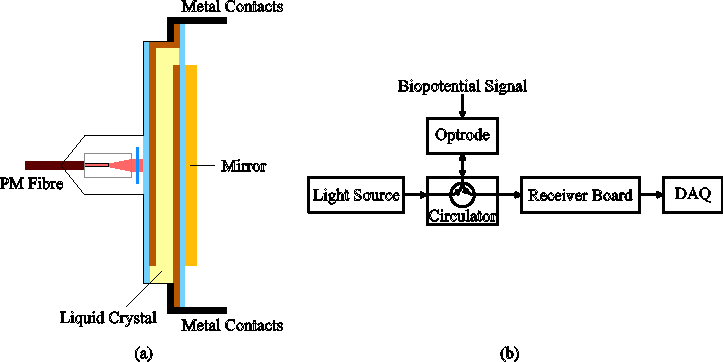
\includegraphics[width=0.9\linewidth]{OptrodeFigure.pdf}}
\caption{(a) Diagram of optrode transducer used in electrophysiological  detection.  Light comes in from Polarization-maintaining (PM) fibre, is rotated by liquid crystal, reflected by the mirror and goes back into the PM fibre. (b) Optrode electrophysiological  detection system block diagram.  Light goes into the optrode from the light source, carries nerve signal, and is converted at the receiver board and DAQ to digital signal.}
\label{fig_OptrodeFigure}
\end{figure}

An optical-electrode or ``optrode'' is a recently developed device for detecting biopotential signals of neuronal, cardiac, or muscular origin.~\cite{OptrodeTransducer}.  Fig.~\ref{fig_OptrodeFigure}(a) shows the structure of such an optrode: light that is generated from a super-luminescent diode light source is guided to the optrode via a polarisation-maintaining fibre (PM fibre).  The polarised light sees its polarisation being rotated by a thin (5\ $\mu$m) layer of liquid crystals by an angle depending on the voltage applied across the metal contacts~\cite{LCVsensor}.  The light is then reflected by the back mirror and returns to the PM fibre where the amount of light recaptured depends on the rotation angle of the liquid crystals. The optrode is designed to create a linear relationship between the light detected and the voltage applied to the metal contacts.

In an existing electrophysiological  detection system such as sketched in Fig.~\ref{fig_OptrodeFigure}(b), the optrode is used to convert neuronal signals into light signals as explained above.  The light intensity recaptured is -- in this case -- modulated by the biopotential signal present at one of the metal contacts (the other one being grounded). The light that comes out from the optrode is then directed to a receiver board where a photodiode converts the light into an analogue electrical signal which is then sampled by the data acquisition equipment.

This system has lower signal attenuation~\cite{OptrodeArray,ImpedanceOfOptrode} compared to conventional electronic detection systems. However, the output noise level of the current system is significantly higher than that of conventional microelectrode-based systems. This means it is harder to observe nerve activity, especially when the signal amplitude is small (less than~\qty{10}{mV}).  In previous experiments, it was observed that most of the noise was coming from the light source and thus, a direct way to reduce noise is to design a low-noise current source~\cite{LowNoiseCurrentSource} to power the light source.  In this project, we propose an additional method to reduce noise: active noise cancelling.

The active noise cancelling technique is used in multiple applications such as noise-cancelling headphones~\cite{ANC_Headphone_1,ANC_Headphone_2}, noise-cancelling in cars~\cite{ANC_Car}, RF signal noise-cancelling~\cite{ANC_RF}, {\em etc}.  The basic principle of active noise cancelling for the sound wave is that when two waves have basically the same frequency and amplitude but opposite phases, they will cancel each other out.  In our case, we are dealing with noise in the digital signal form, which requires filtering techniques rather than just subtracting the two signals.  Wiener filters~\cite{WienerFilter} are widely used in signal processing of active noise cancelling applications {\em e.g.}\cite{ANC_Wiener_2,ANC_Wiener_3}.  Since the nerve signal that the optrode system is detecting has a similar frequency range compared to audible sound frequency, active noise cancelling with Wiener filtering should be effective here as well. Thus we propose herein such an approach which, to the best of our knowledge, has not yet been proposed elsewhere.


\section{Scope of work}

This project aims at designing a active noise cancelling system that reduces the noise level in an existing optrode measurement system. The main outcome of this project is the active noise cancelling system that consists of two board, a light receiver PCB, and an FPGA development board. The project begins with a literature review to active noise cancelling designs, and optrode.  Then we analyzes previous receiver boards and designs a new light receiver board, simulation are run and performance are tested to ensure the circuits on the board work as expected. The heart of the project lies in the development of a noise-cancelling algorithm, starting with the foundational Wiener filter. This filter is then modified and tested first in MATLAB, and then implemented in Verilog HDL, with further explorations into the usage of DSP blocks and final implementation on an FPGA platform.  Experimental sections examine the correlation between different noise signals, compare the performance of the newly designed system with existing technologies, test with sinusoidal signals on optical input, and study the artifacts introduced by physical movements and their impact on signal quality.
